\section{Felanalys}
VHDL-modulen för temperatursensorn har testats noggrant genom att genomföra flera mätningar på olika platser.
Kontroller att temperaturen är koncis med andra temperatursensorer har även genomförts. Se \autoref{fig:temperr} för felmarginalsspecifikationer.

Temperaturmätningen har testats i inomhusmiljö ($\approx 23\degcel$) samt utomhusmiljö ($\approx -10\degcel$) med goda resultat.
Kalibrering av tidsintervall har simulerats samt testats empiriskt för att hitta optimala värden. Den slutgiltiga revisionen är testad upp till ca. 1000 korrekta mätningar i rad, där den kan anses vara helt fungerande.


\begin{figure}[htp]
\centering
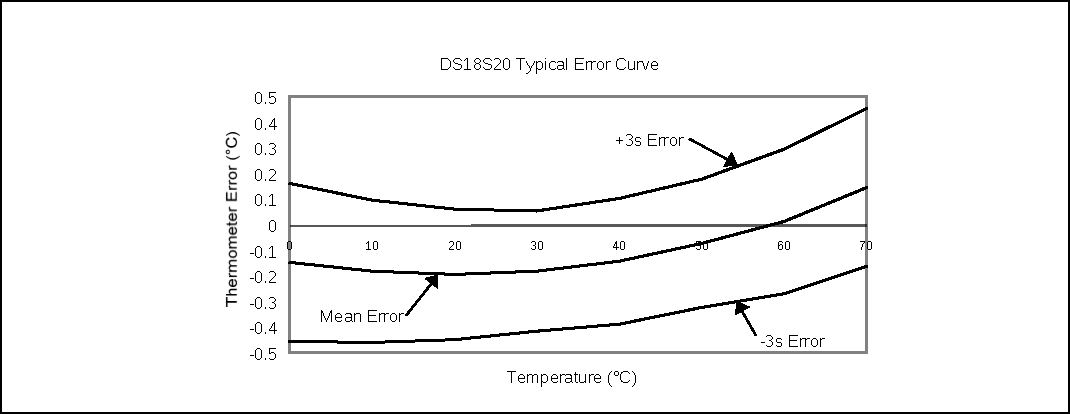
\includegraphics[width=\textwidth]{temp_error.pdf}
\caption{Visar hur DS18S20s mätfel varierar beroende på temperaturförändringar.}
\label{fig:temperr}
\end{figure}